
\section{Model-based Analysis}

As described in the introduction, interactive interfaces must respond within interactive latencies otherwise it will affect user exploration.
However, 
Since the goal is to ensure a consistently low user-perceived latency, we use a simple latency model to
highlight the key factors that affect user-perceived latency.


Let $t$ be the number of milliseconds in the future when the user will make a request.
Let the variables $l_{net,cache,user}$ represent the latency to fetch and render the request from the server,
the latency to render data if it is found in the client cache, and the perceived latency of the user, respectively.
Let $\alpha$ be the accuracy of the prediction model.

Walk through typical numbers for these variables and where they come frome.

$$l_{user} = (l_{cache} + max(0, l_{net} - t)\times \alpha + l_{net}\times(1-\alpha) $$

We use $max()$ because 

Rearranging the terms, we can derive the minimum prediction accuracy in order to maintain $l_{user}$.

$$\alpha = \frac{l_{net} - l_{user}}{l_{net} - l_{cache}}$$

If we set the desired user latency to $100$ milliseconds, then Figure~\ref{fig:model_base} plots the model accuracy as the network latency (x-axis) and \ewu{another factor} (lines).

\begin{figure}
	\centering
	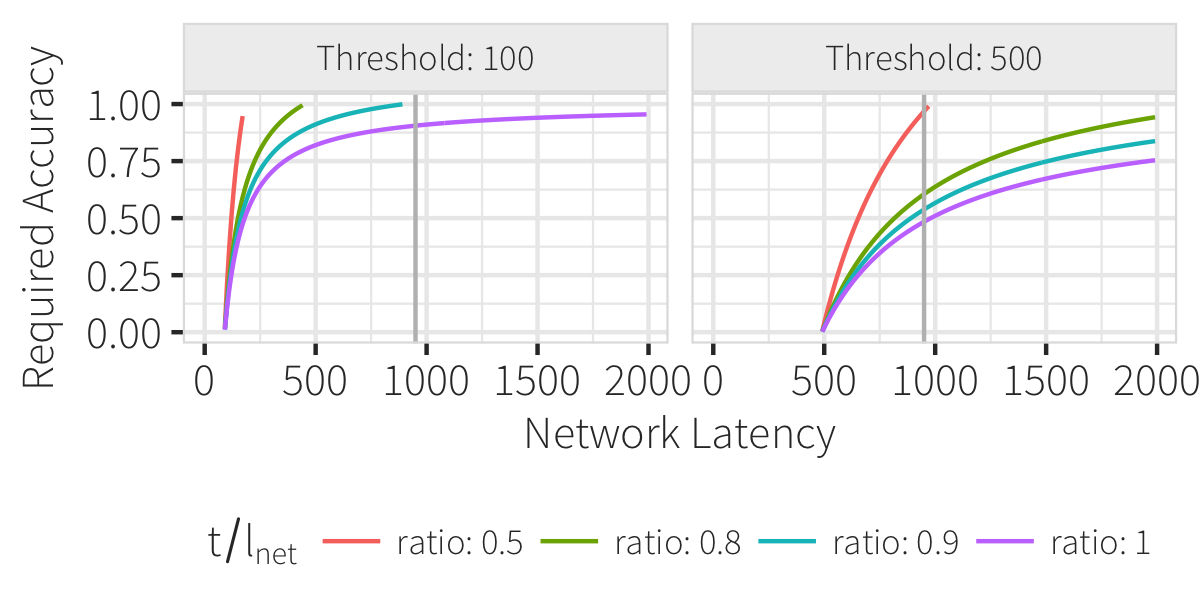
\includegraphics[width=1\columnwidth]{figures/model_base}
 	\caption{Required prediction accuracy as a function of network latency, when look-ahead time $t$ is a fraction of network latency.}
    \label{fig:model_base}
\end{figure}

\begin{figure}
	\centering
	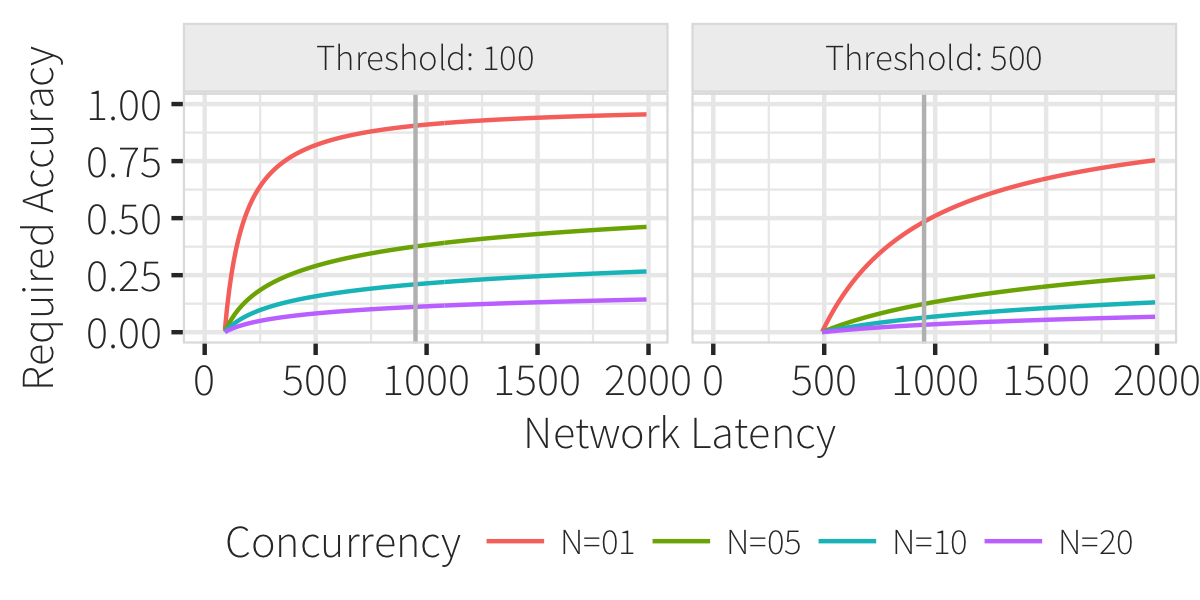
\includegraphics[width=1\columnwidth]{figures/model_concurrency}
 	\caption{Required prediction accuracy as a function of network latency, as concurrency increases (lines) and for two latency thresholds (facets).}
  \label{fig:model_concurrency}
\end{figure}

\begin{figure}
	\centering
	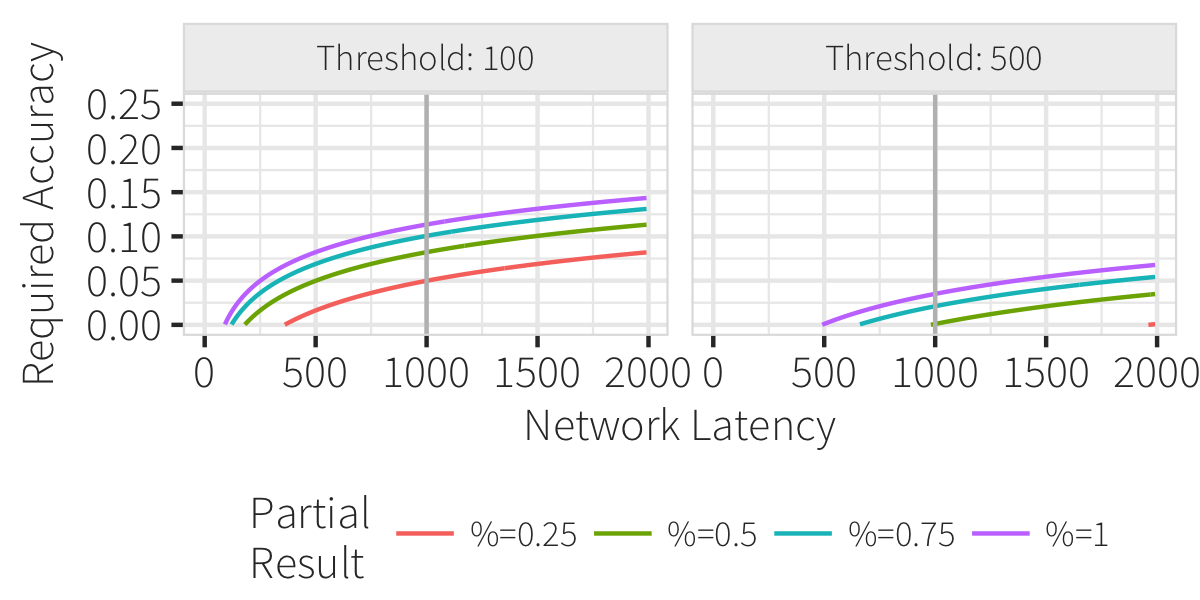
\includegraphics[width=1\columnwidth]{figures/model_partial}
 	\caption{Required prediction accuracy as a function of network latency, under progressive conditions where partial responses are sufficient.}
    \label{fig:model_partial}
\end{figure}



\stitle{Vary Prefetch Concurrency}

\stitle{Vary Perceived Latency Threshold}

\stitle{Network Latency Variance}

\stitle{Progressive Loading}

Assuming a tile is XXX kilobytes, and a throughput of $T mb/s$, then can sustain a concurrency level of XXX.  
When combined with progressive loading of $20\%$ (base this number off sampling and immens arguments), increases the concurrency level to XXX, 
and the model accuracy to YYY.  In many existing settings, where the number of interaction options is limited, this effectively means the prediction model
can draw randomly and be effective.  

However, in interfaces such as XXX, the number of possible interactions are roughly YYY, for which existing techniques would fail.  Under our analysis, the model simply needs to be.



\subsection{Summary of Findings}

